\documentclass[tikz,border=12pt]{standalone}
\usepackage{amsmath,amssymb}
\usetikzlibrary{calc}

\begin{document}
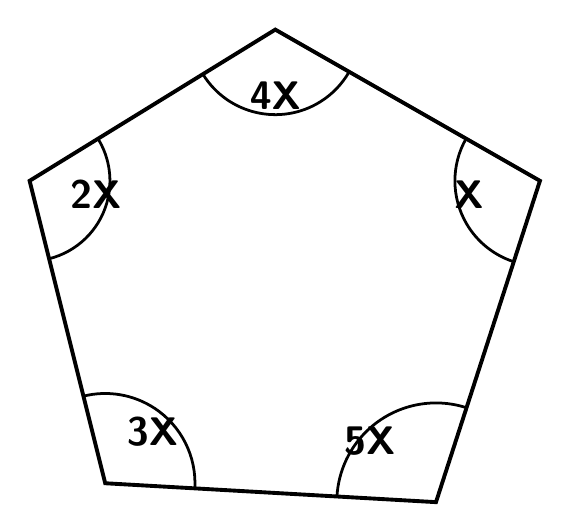
\begin{tikzpicture}[scale=1.2]
    % 5 vertices of the pentagon
    \coordinate (V1) at (0, 3.0);       % 4X (top)
    \coordinate (V2) at (-2.6, 1.4);    % 2X (left)
    \coordinate (V3) at (-1.8, -1.8);   % 3X (bottom-left)
    \coordinate (V4) at (1.7, -2.0);    % 5X (bottom-right)
    \coordinate (V5) at (2.8, 1.4);     % X (right)
    
    % Draw polygon
    \draw[line width=1.4pt] (V1) -- (V2) -- (V3) -- (V4) -- (V5) -- cycle;
    
    % Arcs at each vertex
    % V1: top arc
    \draw[line width=1.0pt] ($(V1) + (212:0.9)$) arc (212:330:0.9);
    \node[font=\Large\sffamily\bfseries] at (0, 2.3) {4X};
    
    % V2: left arc
    \draw[line width=1.0pt] ($(V2) + (284:0.85)$) arc (284:391.6:0.85);
    \node[font=\Large\sffamily\bfseries] at (-1.9, 1.25) {2X};
    
    % V3: bottom-left arc
    \draw[line width=1.0pt] ($(V3) + (-3.3:0.95)$) arc (-3.3:104:0.95);
    \node[font=\Large\sffamily\bfseries] at (-1.3, -1.25) {3X};
    
    % V4: bottom-right arc
    \draw[line width=1.0pt] ($(V4) + (72:1.05)$) arc (72:176.7:1.05);
    \node[font=\Large\sffamily\bfseries] at (1.0, -1.35) {5X};
    
    % V5: right arc
    \draw[line width=1.0pt] ($(V5) + (150.3:0.9)$) arc (150.3:252:0.9);
    \node[font=\Large\sffamily\bfseries] at (2.05, 1.25) {X};
    
\end{tikzpicture}
\end{document}
